\newpage
\subsection{Xác minh chữ ký}

\subsubsection*{Mục tiêu}
Chức năng xác minh chữ ký cho phép người dùng kiểm tra tính toàn vẹn và nguồn gốc của một tập tin bất kỳ thông qua file chữ ký `.sig` do người gửi tạo ra. Việc xác minh này giúp đảm bảo:
\begin{itemize}
    \item Tập tin không bị chỉnh sửa sau khi ký.
    \item Người nhận có thể xác định chính xác ai là người ký.
    \item Thời điểm ký được xác minh và hiển thị lại rõ ràng.
\end{itemize}

\subsubsection*{Giao diện}
Giao diện xác minh tại trang \texttt{/crypto/verify} bao gồm:
\begin{itemize}
    \item Trường upload 2 file: tập tin gốc cần xác minh và file chữ ký `.sig`.
    \item Nút “Xác minh chữ ký” gửi yêu cầu lên server bằng \texttt{fetch()}.
    \item Kết quả xác minh hiển thị thông tin người ký và thời điểm ký nếu hợp lệ.
    \item Toast thông báo xác minh thành công hoặc thất bại.
\end{itemize}

\begin{figure}[H]
    \centering
    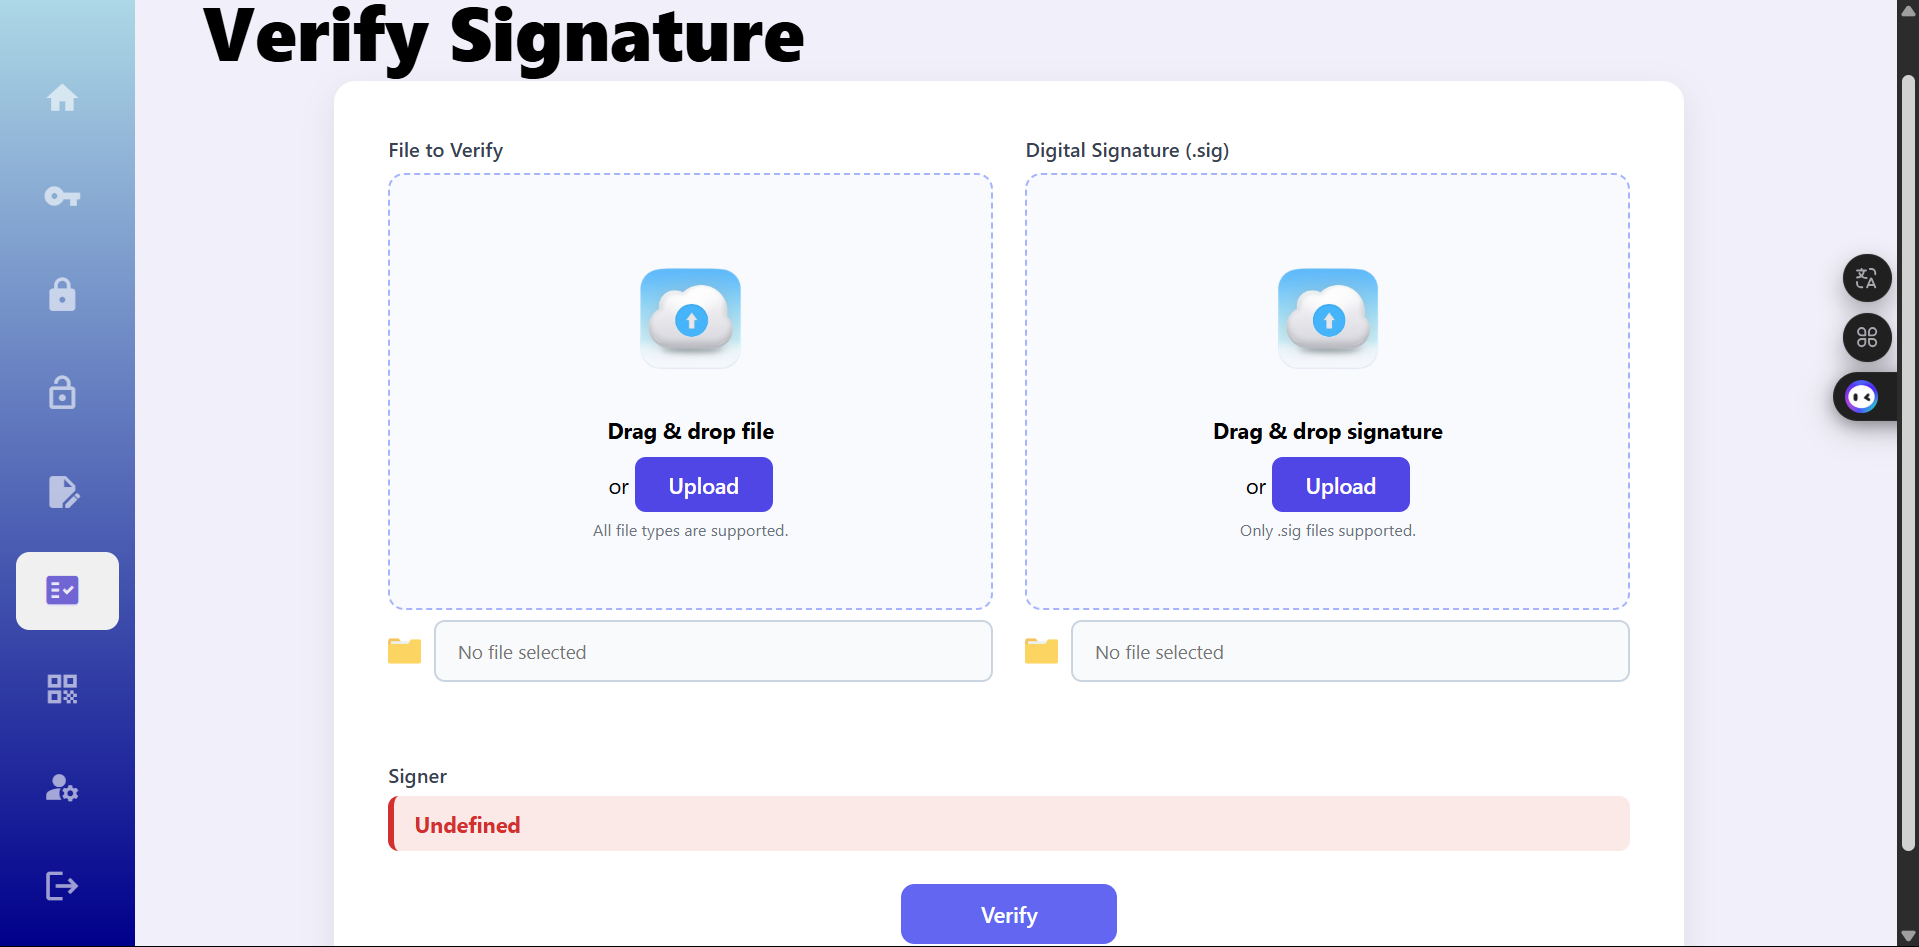
\includegraphics[width=0.85\textwidth]{img/9_verify/9_verify_form.png}
    \caption{Giao diện xác minh ký số}
\end{figure}

\subsubsection*{Quy trình thực hiện}

\begin{description}
    \item[\textbf{Bước 1 - Frontend:}] Người dùng chọn tập tin và file chữ ký `.sig`, sau đó gửi lên server bằng \texttt{FormData}.
    \begin{itemize}
        \item Gửi POST đến \texttt{/utils/verify\_signature}.
        \item Gửi kèm 2 trường: \texttt{file\_to\_verify} và \texttt{signature}.
        \item Nếu kết quả hợp lệ → hiển thị tên người ký và thời điểm ký.
    \end{itemize}

    \begin{figure}[H]
        \centering
        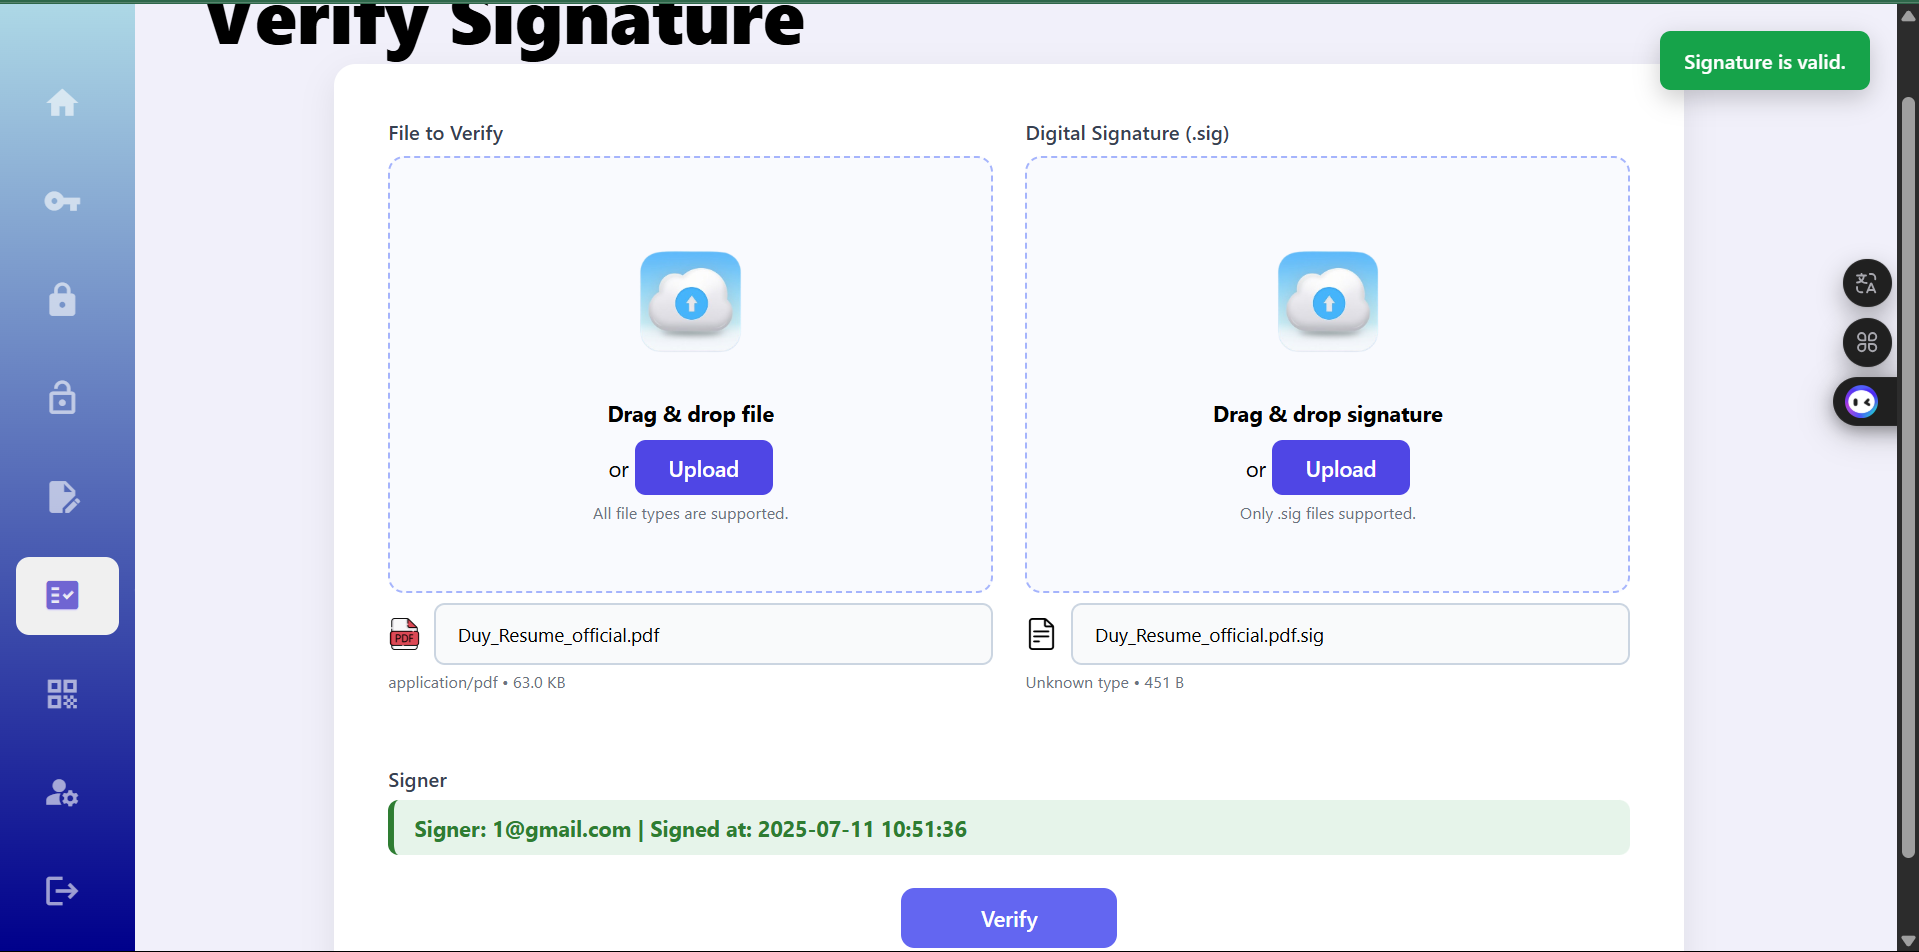
\includegraphics[width=0.85\textwidth]{img/9_verify/9_verify_success.png}
        \caption{Xác minh ký số thành công}
    \end{figure}

    \begin{figure}[H]
        \centering
        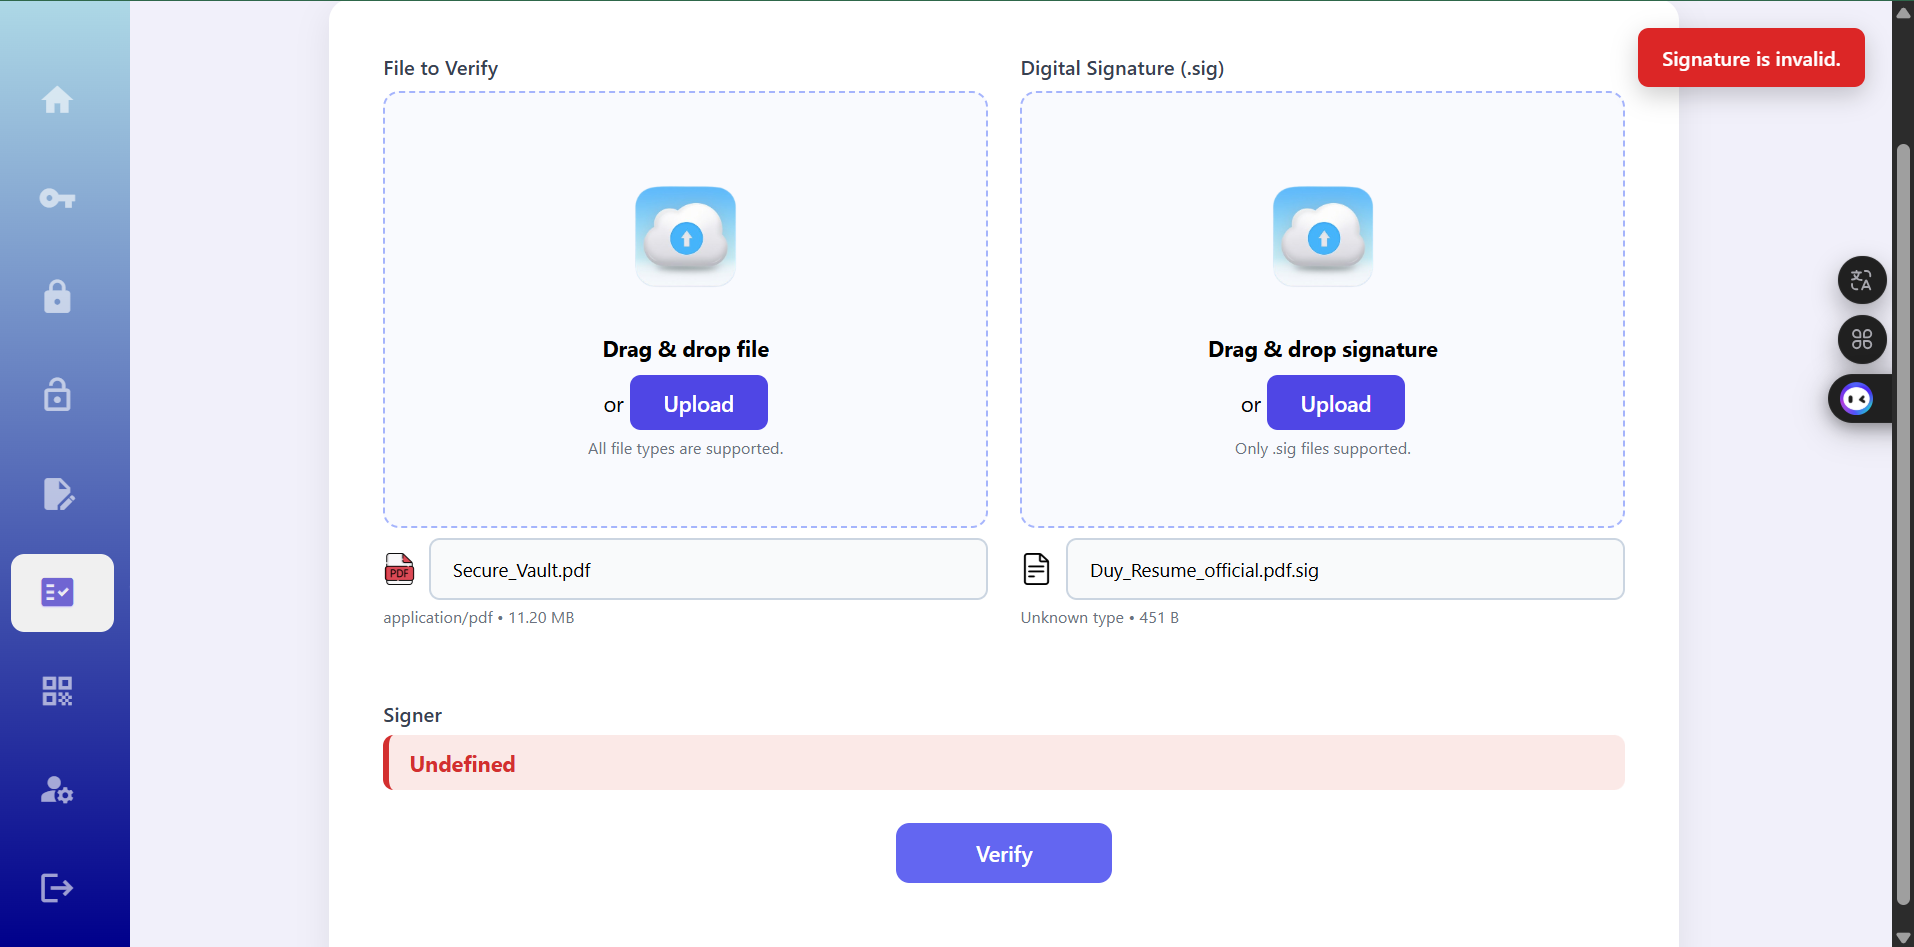
\includegraphics[width=0.85\textwidth]{img/9_verify/9_verify_invalid.png}
        \caption{Chữ ký không được xác minh}
    \end{figure}

    \item[\textbf{Bước 2 - Flask Route:}] Route xử lý tại \texttt{/verify\_signature}.
    \begin{enumerate}
        \item Kiểm tra session và sự tồn tại của cả 2 file.
        \item Đọc nội dung file chữ ký và parse JSON.
        \item Đọc danh sách public key từ file \texttt{contact\_public\_key.json}.
        \item Gọi hàm \texttt{verify\_signature(...)} để xác minh chữ ký.
        \item Ghi log kết quả (thành công hoặc thất bại) và trả về thông tin người ký.
    \end{enumerate}

    \item[\textbf{Bước 3 - Xử lý xác minh (Modules):}] Hàm \texttt{verify\_signature()} thực hiện:
    \begin{enumerate}
        \item Tính hash SHA-256 của tập tin gốc.
        \item Dò từng public key trong danh sách để thử xác minh.
        \item Nếu khớp → trả về email người ký và thời gian.
        \item Nếu không khớp → trả lỗi “Signature is invalid”.
    \end{enumerate}
\end{description}

\subsubsection*{Chi tiết kỹ thuật và thư viện bảo mật}

\begin{description}

    \item[\textbf{1. Phân tích file chữ ký:}]
    File chữ ký `.sig` là JSON chứa chữ ký (dạng base64) và timestamp. Hệ thống decode và parse dữ liệu để chuẩn bị xác minh.
    \begin{itemize}
        \item Đọc bằng \texttt{.read().decode('utf-8')} và xử lý JSON với \texttt{json.loads(...)}.
        \item Giải mã chữ ký với \texttt{base64.b64decode(...)}.
    \end{itemize}

    \item[\textbf{2. Duyệt danh sách public key:}]
    Server đọc file \texttt{contact\_public\_key.json} chứa public key của các người gửi.
    \begin{itemize}
        \item Public key lưu dưới dạng PEM, được parse bằng \texttt{serialization.load\_pem\_public\_key()}.
        \item Với mỗi key, thử gọi \texttt{public\_key.verify(...)} để kiểm tra.
    \end{itemize}

    \item[\textbf{3. Tính hash và xác minh:}]
    Server tính hash SHA-256 của file gốc và dùng RSA-PKCS1v15 để xác minh chữ ký.
    \begin{itemize}
        \item Hash bằng: \texttt{hashlib.sha256(file\_data).digest()}.
        \item Padding: \texttt{PKCS1v15()}, Hash: \texttt{SHA256()}.
        \item Nếu đúng → xác minh thành công và log email + timestamp.
    \end{itemize}

    \item[\textbf{4. Xử lý lỗi và bảo mật:}]
    Hệ thống có các bước kiểm tra và log lỗi đầy đủ:
    \begin{itemize}
        \item Báo lỗi nếu thiếu file, sai định dạng hoặc không tìm thấy key.
        \item Ghi log bằng \texttt{log\_user\_action()} và \texttt{log\_internal\_event()} theo mức độ \texttt{info}, \texttt{warning}, hoặc \texttt{error}.
        \item Không lưu lại nội dung file, chỉ log metadata để đảm bảo riêng tư.
    \end{itemize}

    \item[\textbf{5. Xử lý lỗi và báo lỗi chi tiết:}]
    Hệ thống được thiết kế để phát hiện và phản hồi rõ ràng với các lỗi có thể xảy ra trong quá trình xác minh chữ ký, đồng thời ghi log đầy đủ theo từng tình huống cụ thể.
    \begin{itemize}
        \item \textbf{Kiểm tra đăng nhập:} Nếu session không tồn tại, trả về mã lỗi \texttt{401} cùng thông báo: \texttt{"You must be logged in to access this page."}.
        \item \textbf{Thiếu file:} Nếu người dùng không gửi cả file cần xác minh hoặc file chữ ký → trả lỗi \texttt{400} kèm thông báo: \texttt{"No file or signature provided"}.
        \item \textbf{Tên file trống:} Nếu \texttt{file.filename == ""} → trả lỗi \texttt{400} với thông báo: \texttt{"Tên file trống"}.
        \item \textbf{Lỗi định dạng chữ ký:}
        \begin{itemize}
            \item Nếu không đọc hoặc decode được nội dung file chữ ký JSON → trả lỗi \texttt{400}, thông báo: \texttt{"Invalid signature file format"}.
            \item Log lỗi này ở mức \texttt{error} vì có thể liên quan đến file bị sửa hoặc không hợp lệ.
        \end{itemize}
        \item \textbf{Thiếu danh sách public key:}
        \begin{itemize}
            \item Nếu không tồn tại file \texttt{contact\_public\_key.json} → trả lỗi \texttt{400} với thông báo: \texttt{"Public key does not exist."}.
            \item Lỗi được log lại kèm tên người dùng để hỗ trợ debug.
        \end{itemize}
        \item \textbf{Chữ ký không hợp lệ:}
        \begin{itemize}
            \item Nếu không có public key nào xác minh được chữ ký → trả lỗi \texttt{400} với thông báo: \texttt{"Signature is invalid."}.
            \item Thông tin file được log kèm để phục vụ điều tra.
        \end{itemize}
        \item \textbf{Log chi tiết:} Mỗi lỗi đều được ghi bằng \texttt{log\_user\_action(...)} với trạng thái \texttt{"Fail"} và ghi rõ lý do, đồng thời có thể bổ sung thêm \texttt{log\_internal\_event()} để phân tích kỹ thuật.
    \end{itemize}

    \begin{figure}[H]
        \centering
        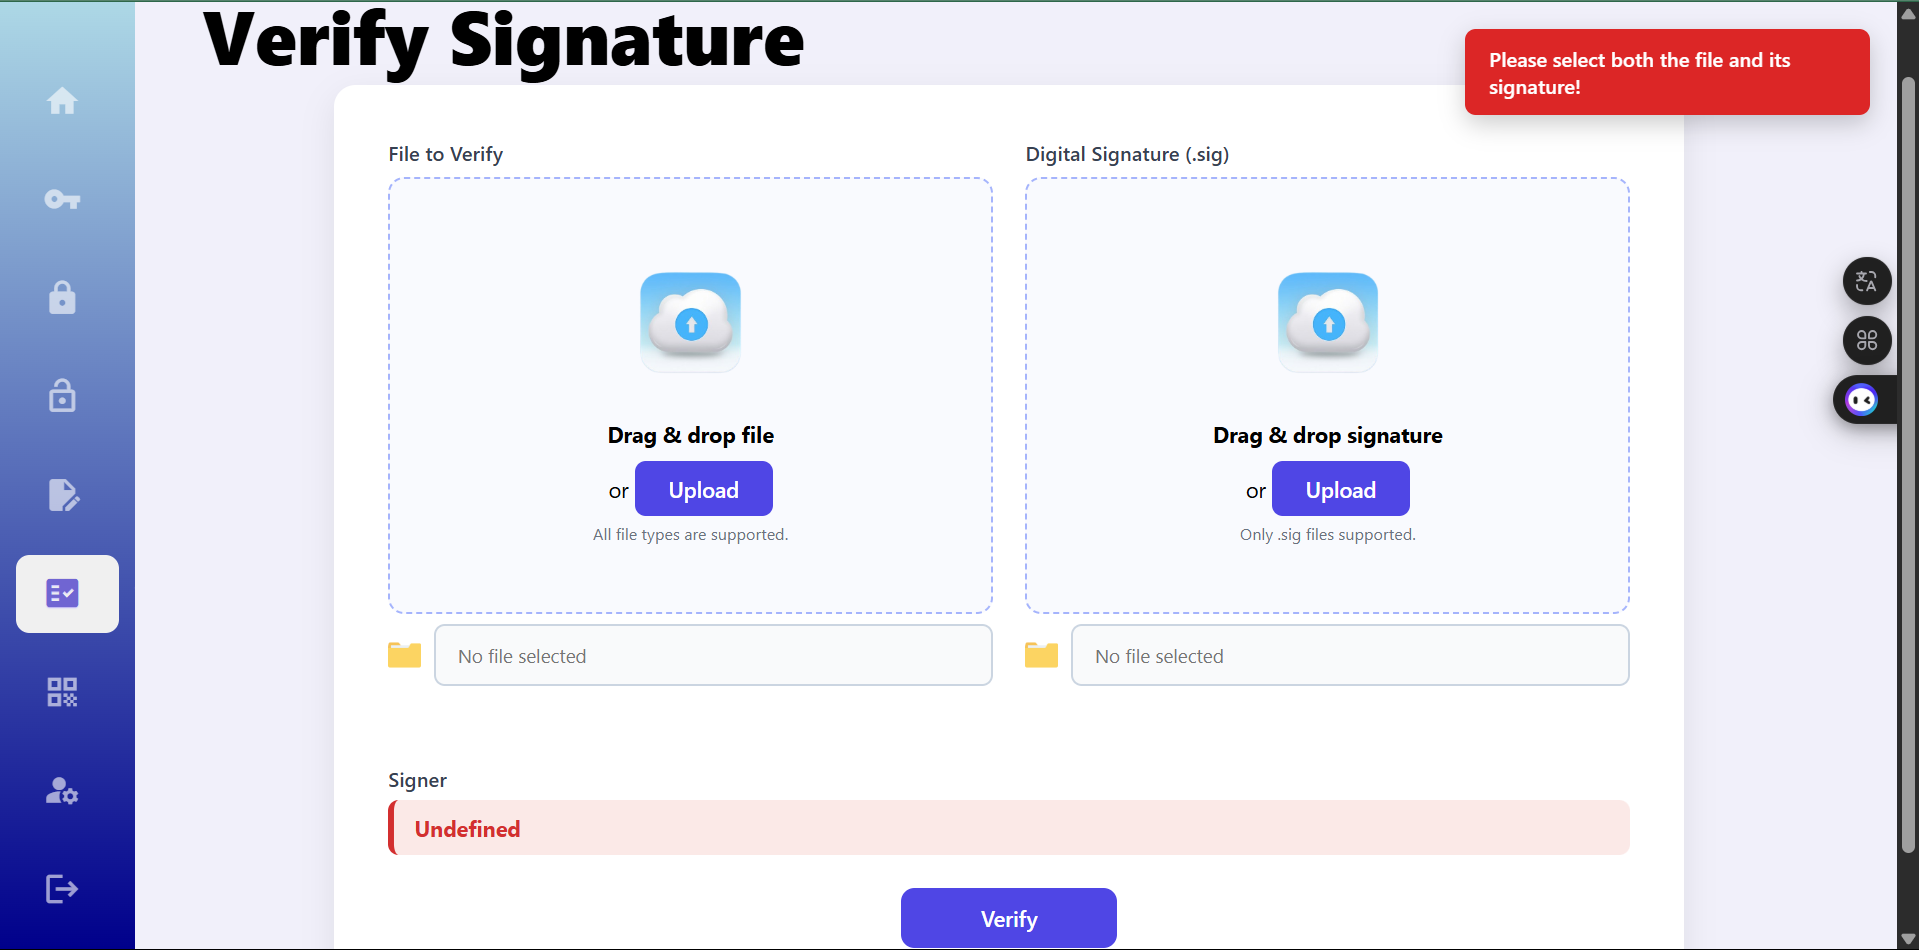
\includegraphics[width=0.85\textwidth]{img/9_verify/9_verify_no_files.png}
        \caption{Kiểm tra có đủ file đầu vào}
    \end{figure}

\end{description}
